

\section{Results}
\label{sec:results}


	\noindent \textbf{Issues with PD controllers:}
	
	Find the right settings for the PD controllers has been a difficult task. This can be linked to difficulties using the \Featherstone algorithm. Typically, the torques on links are applied individually, this is not true in this version of the \Featherstone algorithm. No Link operates independently and any torque applied to a motor at a joint is applied to both links attached at the joint. This issue tends to propagate through the hierarchical chain of links. 
	
	\noindent \textbf{Use Dampening?}
	
	I did try to reduce some issues by applying additional linear and angular dampening. Adding dampening only decreased the effect of the issues, they are still present.
	
	\noindent \textbf{Joint angle specification:}
	
	I found it was also difficult to work with joint angle specification in \bulletPhysics. Joint angles are constrained to be $0 \geq \theta \geq 2*\pi $. When a joint angle would wrap around the PD controller would switch its driving direction. This typically results in the character gaining a significant amount of energy.
	
	\noindent \textbf{Detecting foot to ground contact:}
	
	Currently there are some issues with accurately detecting foot to ground contact. Ground contact is detected earlier than it should be. Investigation into the \bulletPhysics should lead to a solution to this issue.
	
	\noindent \textbf{Issues with defining the torso torque:}
	
	Again, because torques are automatically applied to both links applying \torqueTorso is problematic. The method use in this work was to not specifically apply the torque to the torso but to instead only include it in stance leg torque computation.
	
	
	\noindent \textbf{Some simple walking motion:}
	
	Figure~\ref{figure:algorithm-steps} shows a sequence of the animation in $6$ clips. I think the character would be accepted into the SillyWalk school.
	
	\begin{figure}[!htb]
	\centering
	%trim=l b r t
	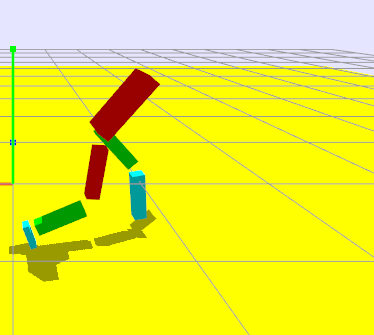
\includegraphics[width=0.45\linewidth]{../images/stepping/step-0.png} 
	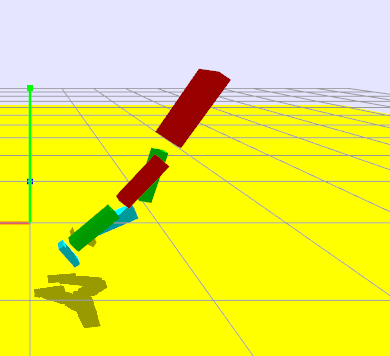
\includegraphics[width=0.45\linewidth]{../images/stepping/step-1.png} \\ 
	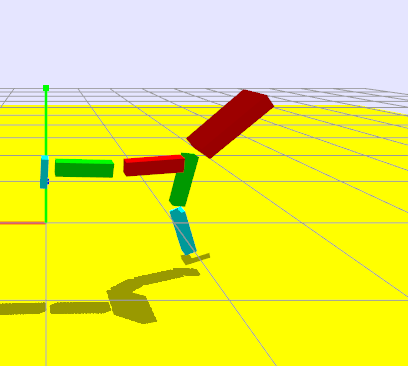
\includegraphics[width=0.45\linewidth]{../images/stepping/step-2.png}  
	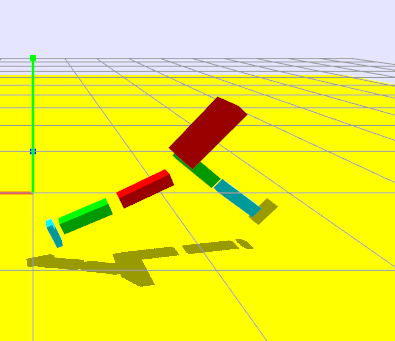
\includegraphics[width=0.45\linewidth]{../images/stepping/step-3.png}  \\
	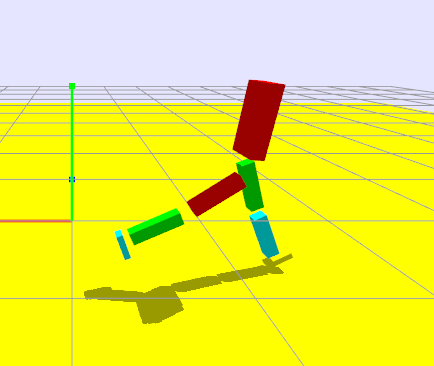
\includegraphics[width=0.45\linewidth]{../images/stepping/step-4.png}  
	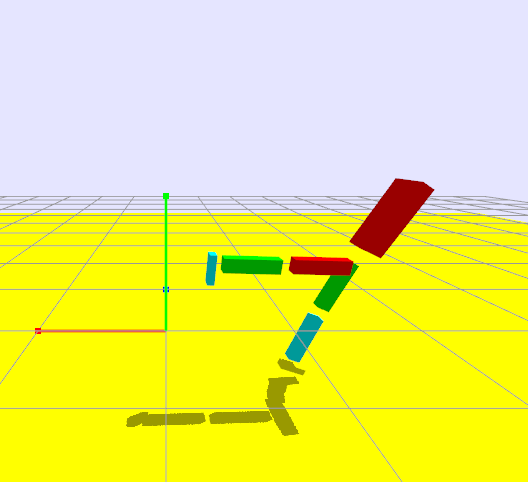
\includegraphics[width=0.45\linewidth]{../images/stepping/step-5.png}

	% \includegraphics[width=0.45\linewidth]{../images/steps/initial-mesh.pdf}  
	% (e) & (f) & (g) & (h)\\
	\caption{\label{figure:algorithm-steps} Sequence of captures of attempted walking behaviour. Order starts in the top left and proceeds to the right and then down.}
	\end{figure}
	
	\begin{figure}
		
	\end{figure}
